\documentclass[tikz]{standalone}
\usepackage{booktabs}
\usepackage{multirow}
\usepackage{times}
\usepackage{sourcecodepro}

\usetikzlibrary{arrows.meta, decorations.pathreplacing, positioning, shapes.misc}
\tikzset{
  na/.style = {baseline=-.75ex},
  every picture/.append style={remember picture},
  every node/.append style={font=\footnotesize},
}

\begin{document}
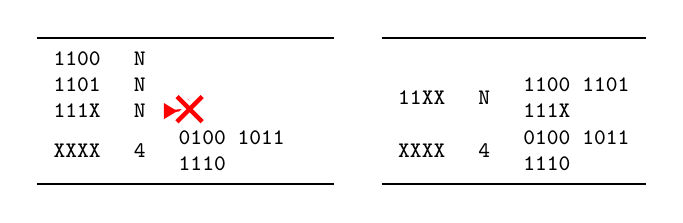
\begin{tikzpicture}
  % Original table
  \node (original) {
    \begin{tabular}{c l l r}
      \toprule
      \texttt{1100} & \texttt{N} & & \tikz[na]\node [coordinate] (e0) {}; \\
      \texttt{1101} & \texttt{N}\\
      \texttt{111X} & \texttt{N} & & \tikz[na]\node [coordinate] (e1) {}; \\
      \multirow{2}{*}{\texttt{XXXX}} &
      \multirow{2}{*}{\texttt{4}} & \texttt{0100 1011}\\
                     &            & \texttt{1110}\\
      \bottomrule
    \end{tabular}
  };

  % Table after merging
  \node (invalid) [right=1em of original] {
    \begin{tabular}{c l l}
      \toprule
      \\
      \multirow{2}{*}{\tikz[na]\node [coordinate] (e2) {};\texttt{11XX}} &
      \multirow{2}{*}{\texttt{N}} & \texttt{1100 1101} \\
                                                        &            & \texttt{111X} \\
      \multirow{2}{*}{\texttt{XXXX}} &
      \multirow{2}{*}{\texttt{4}} & \texttt{0100 1011}\\
                     &            & \texttt{1110}\\
      \bottomrule
    \end{tabular}
  };

  % Add some arrows
  \draw [red, thick, decoration={brace}, decorate] ([yshift=+1ex] e0) -- ([yshift=-.5ex] e1)
    node [midway, coordinate] (merge) {};
  \draw [red, thick, out=0, in=180, arrows={-Triangle[]}, shorten >=3pt] ([xshift=2pt] merge) to
    node [pos=.4, cross out, draw=white, line width=4pt, minimum size=.75em, shorten >=0pt] {}
    node [pos=.4, cross out, draw=red, ultra thick, minimum size=.75em, shorten >=0pt] {}
    (e2);
\end{tikzpicture}
\end{document}
